\documentclass[11pt]{article}
\usepackage{setspace}
\setstretch{1}
\usepackage[T1]{fontenc}
\usepackage{amsmath,amssymb, amsthm}
\usepackage{graphicx}
\usepackage{bm}
\usepackage[hang, flushmargin]{footmisc}
\usepackage[colorlinks=true]{hyperref}
\usepackage[nameinlink]{cleveref}
\usepackage{footnotebackref}
\usepackage{url}
\usepackage{listings}
\usepackage[most]{tcolorbox}
\usepackage{inconsolata}
\usepackage[papersize={8.5in,11in}, margin=1in]{geometry}
\usepackage{float}
\usepackage{caption}
\usepackage{esint}
\usepackage{url}
\usepackage{enumitem}
\usepackage{subfig}
\usepackage{wasysym}
\newcommand{\ilc}{\texttt}
\usepackage{etoolbox}
\usepackage{algorithm}
% \usepackage{algorithmic}
\usepackage[noend]{algpseudocode}
\usepackage{tikz}
\usetikzlibrary{matrix,positioning,arrows.meta,arrows}
\patchcmd{\thebibliography}{\section*{\refname}}{}{}{}

\makeatletter
\renewcommand{\@seccntformat}[1]{}
\makeatother


\begin{document}



\title{\textbf{EECS 340: Assignment 4}}

\author{Shaochen (Henry) ZHONG, \ilc{sxz517} \\ Yuhui ZHANG, \ilc{yxz2052}}
\date{Due and submitted on 03/19/2020 \\ EECS 340, Dr. Koyut{\"u}rk}
\maketitle

% % % % % % % % % % % % % % % % % % % % % % % % % % % % % % % % % %
% % % % % % % % % % % % % % % % % % % % % % % % % % % % % % % % % %
% % % % % % % % % % % % % % % % % % % % % % % % % % % % % % % % % %
\section{Problem 1}

\begin{figure}[H]
    \centering
    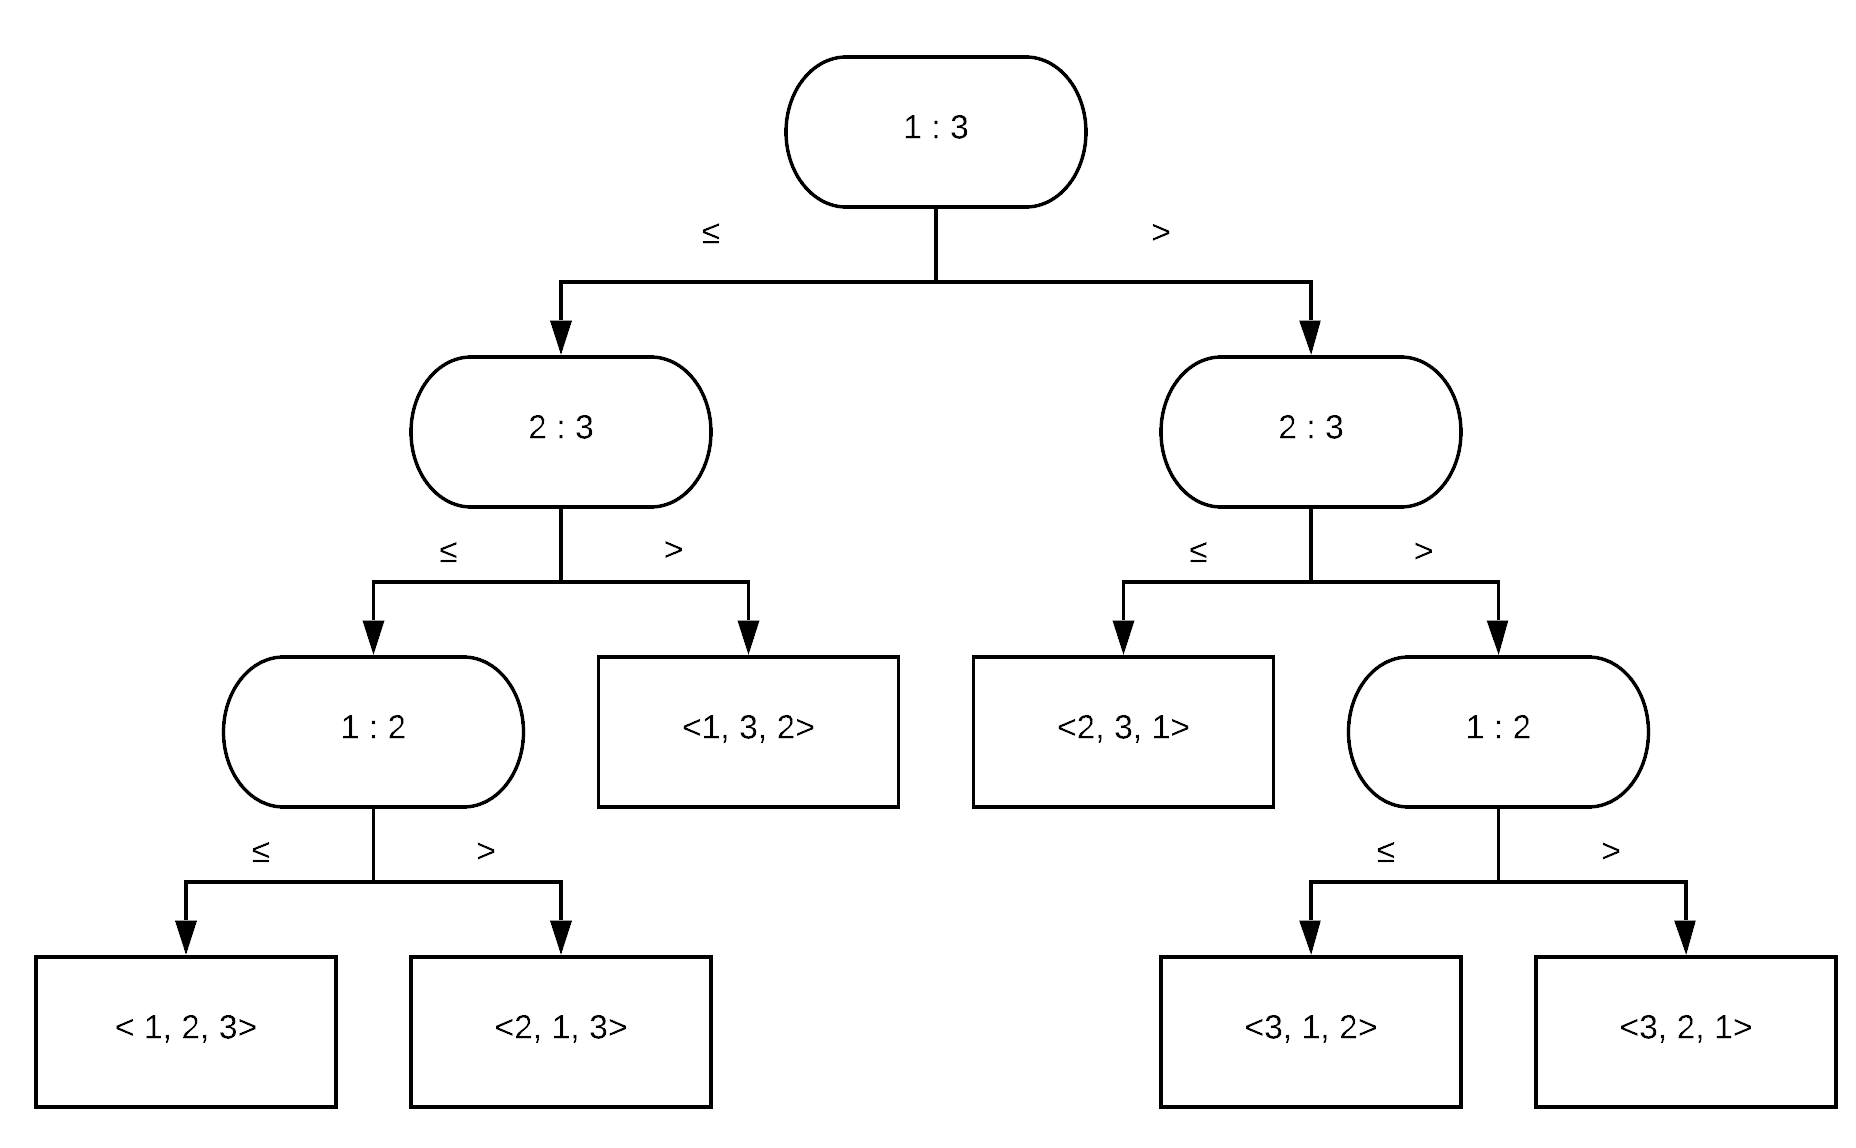
\includegraphics[width=0.8\linewidth]{{fig/fig_1.png}}
    \caption{Decision Tree of \textsc{Quicksort}}
    \label{fig:1}
\end{figure}

% % % % % % % % % % % % % % % % % % % % % % % % % % % % % % % % % %
% % % % % % % % % % % % % % % % % % % % % % % % % % % % % % % % % %
% % % % % % % % % % % % % % % % % % % % % % % % % % % % % % % % % %
\section{Problem 2}

\subsection{Procedure \textsc{PreProcess}(A)}

\begin{algorithm}[H]
\caption{PreProcess(A)}\label{PreProcess}
    \begin{algorithmic}[1]
        \Procedure{PreProcess}{A, p, r}
        \State \text{Let $C[0, 1, ..., k]$ be an arry of $0$.}
        \For {$i \gets 0$ \textbf{to} $n$}
            \State $C[A[i]] = C[A[i]] + 1$
        \EndFor
        \For {$j \gets 1$ \textbf{to} $k$}
            \State $C[j] = C[j] + C[j-1]$
        \EndFor
        \State \Return $C$
        \EndProcedure
    \end{algorithmic}
\end{algorithm}

\subsection{Procedure \textsc{Query}(A, a, b)}

\begin{algorithm}[H]
\caption{Query(A, a, b)}\label{Query}
    \begin{algorithmic}[1]
        \Procedure{Query}{A, a, b}
        \If {$a == 0$}
            \State \Return $A[b]$
        \Else
            \State \Return $A[b] - A[a-1]$
        \EndIf
        \EndProcedure
    \end{algorithmic}
\end{algorithm}

% % % % % % % % % % % % % % % % % % % % % % % % % % % % % % % % % %
% % % % % % % % % % % % % % % % % % % % % % % % % % % % % % % % % %
% % % % % % % % % % % % % % % % % % % % % % % % % % % % % % % % % %
\section{Problem 3}


This probably not the most reader-friendly pseudocode you'd see, but the idea behind it is very intuitive. Thus, I'd like to keep this design, and I'll give many comments to navigate you through my train-of-logic.

\begin{algorithm}[H]
\caption{Sparse-Transpose(R, C, V, m, n, k)}\label{transpose}
    \begin{algorithmic}[1]
        \Procedure{Sparse-Transpose}{A, a, b}
        \State \text{Let $CH[0, 1, ..., n]$ be an arry of $0$.} \Comment{Value holder array.}
        \State \text{Let $VH[0, 1, ..., n]$ be an arry of $0$.} \Comment{Column index holder array.}
        \For {$i \gets 0$ \textbf{to} $n$}
            \State $start \gets R[i]$ \Comment{Calculate the row index of element in C}
            \State $end \gets R[i+1]-1$
            \State \text{Let $CPR[\ ]$ be an empty array.}
            \State \text{Let $VPR[\ ]$ be an empty array.}
            \For {$j \gets start$ \textbf{to} $end$}
                \State $CPR[i].append(C[j])$ \Comment{Holds column indexs according to their row index.}
                \State $VPR[i].append(V[j])$ \Comment{Holds values according to their row index.}
            \EndFor
            \State $CH[i].append(CPR)$ \Comment{$CH[i]$ represents the column index of elements on i-th row.}
            \State $VH[i].append(VPR)$ \Comment{$VH[i]$ represents the value of elements on i-th row.}
        \EndFor
        \State \text{Let $R'[\ ]$ be an empty array.}
        \State \text{Let $C'[\ ]$ be an empty array.}
        \State \text{Let $V'[\ ]$ be an empty array.}
        \State $R'.append(0)$ \Comment{To fill-in the extra element as $len(R') = m + 1$.}
        \State \text{Let $len\_max$ to be the max len of all elements in $CH$}. \Comment{Row with most elements.}
        \For {$i \gets 0$ \textbf{to} $len\_max$}
            \State $\textsc{Pop-Smallest}(R', C', V', CH, VH, len\_max)$ \Comment{Pop the original row index/value to $C'/V'$ of an element with smallest column index.}
        \EndFor
        \For {$i \gets 1$ \textbf{to} $n$}
            \State $R'[i] = R'[i] + R'[i-1]$
        \EndFor
        \State \Return $R', C', V'$
        \EndProcedure
    \end{algorithmic}
\end{algorithm}

\begin{algorithm}[H]
\caption{Pop-Smallest(R, C, V, CH, VH, len\_max)}\label{pop}
    \begin{algorithmic}[1]
        \Procedure{Pop-Smallest}{R, C, V, CH, VH, len\_max}
        \State $min\_value \gets CH[0][0]$ \Comment{Assume 1st element on row 1 is the one with smallest column index.}
        \State $min\_i \gets 0$
        \State $min\_j \gets 0$
        \For {$i \gets 0$ \textbf{to} $len\_max$} \Comment{Iterate all elements' column index on a particular row.}
            \State $R\_counter \gets 0$ \Comment{Check if elements with same column index on multiple rows.}
            \For {$j \gets 0$ \textbf{to} $n$} \Comment{Interate all rows registered in $CH$}
                \If {$CH[j][i] == min\_value$} \Comment{If current element has the same column index}
                    \State $R\_counter \gets R\_counter + 1$ \Comment{Update R'.}
                    \If {$j < min\_j$} \Comment{If current element also has smaller row index than the holder.}
                        \State $min\_value \gets CH[j][i]$ \Comment{Update holders.}
                        \State $min\_i \gets i$
                        \State $min\_j \gets j$
                    \EndIf
                \EndIf
                \If {$CH[j][i] < min\_value$}  \Comment{If current elements column index is smaller than the holder.}
                    \State $R\_counter \gets R\_counter + 1$
                    \State $min\_value \gets CH[j][i]$ \Comment{Update holders.}
                    \State $min\_i \gets i$
                    \State $min\_j \gets j$
                    \State \text{continue}
                \EndIf

            \EndFor
            \State $CH[min\_j].remove(min\_i)$ \Comment{Pop the element with smallest column index.}
            \State $C.append(min\_j)$ \Comment{Append element with smallest column index's row index.}
            \State $V.append(VH[min\_j][min\_i])$ \Comment{Append element's corresponding value.}
            \State $VH[min\_j].remove(min\_i)$ \Comment{Pop such value.}
            \State $R.append(R\_counter)$ \Comment{Register how many elements on each column.}
        \EndFor
    \end{algorithmic}
\end{algorithm}

The algorithm is considered $O(m + n + k)$ as the \ilcode{line 4-6} in \textsc{Sparse-Transpose} needs $O(m)$, loop through of C, V needs $O(k)$, and loop through of $R'$ needs $O(n)$.
% \section{References}
%
% \nocite{*}
% \raggedright
% \bibliography{references.bib}
% \bibliographystyle{plain}


\end{document}